%----------------------------------------------------------------------------------------

\documentclass[a4paper,10pt]{article} % Uses article class in A4 format

%----------------------------------------------------------------------------------------
%	FORMATTING
%----------------------------------------------------------------------------------------

\setlength{\parskip}{0pt}
\setlength{\parindent}{0pt}
\setlength{\voffset}{-15pt}

%----------------------------------------------------------------------------------------
%	PACKAGES AND OTHER DOCUMENT CONFIGURATIONS
%----------------------------------------------------------------------------------------

\usepackage[a4paper, margin=2.5cm]{geometry} % Sets margin to 2.5cm for A4 Paper
\usepackage[onehalfspacing]{setspace} % Sets Spacing to 1.5

\usepackage[T1]{fontenc} % Use European encoding
\usepackage[utf8]{inputenc} % Use UTF-8 encoding
\usepackage{charter} % Use the Charter font
\usepackage{microtype} % Slightly tweak font spacing for aesthetics

\usepackage[english]{babel} % Language hyphenation and typographical rules

\usepackage{amsthm, amsmath, amssymb} % Mathematical typesetting
\usepackage{marvosym, wasysym} % More symbols
\usepackage{float} % Improved interface for floating objects
\usepackage[final, colorlinks = true, 
            linkcolor = black, 
            citecolor = black,
            urlcolor = black]{hyperref} % For hyperlinks in the PDF
\usepackage{graphicx, multicol} % Enhanced support for graphics
\usepackage{xcolor} % Driver-independent color extensions
\usepackage{rotating} % Rotation tools
\usepackage{listings, style/lstlisting} % Environment for non-formatted code, !uses style file!
\usepackage{pseudocode} % Environment for specifying algorithms in a natural way
\usepackage{style/avm} % Environment for f-structures, !uses style file!
\usepackage{booktabs} % Enhances quality of tables

\usepackage{tikz-qtree} % Easy tree drawing tool
\tikzset{every tree node/.style={align=center,anchor=north},
         level distance=2cm} % Configuration for q-trees
\usepackage{style/btree} % Configuration for b-trees and b+-trees, !uses style file!

\usepackage{titlesec} % Allows customization of titles
\renewcommand\thesection{\arabic{section}.} % Arabic numerals for the sections
\titleformat{\section}{\large}{\thesection}{1em}{}
\renewcommand\thesubsection{\alph{subsection})} % Alphabetic numerals for subsections
\titleformat{\subsection}{\large}{\thesubsection}{1em}{}
\renewcommand\thesubsubsection{\roman{subsubsection}.} % Roman numbering for subsubsections
\titleformat{\subsubsection}{\large}{\thesubsubsection}{1em}{}

\usepackage[all]{nowidow} % Removes widows

\usepackage[backend=biber,style=numeric,
            sorting=nyt, natbib=true]{biblatex} % Complete reimplementation of bibliographic facilities
\addbibresource{main.bib}
\usepackage{csquotes} % Context sensitive quotation facilities

\usepackage[yyyymmdd]{datetime} % Uses YEAR-MONTH-DAY format for dates
\renewcommand{\dateseparator}{-} % Sets dateseparator to '-'

\usepackage{fancyhdr} % Headers and footers
\pagestyle{fancy} % All pages have headers and footers
\fancyhead{}\renewcommand{\headrulewidth}{0pt} % Blank out the default header
\fancyfoot[L]{\textsc{Robin Worreby}} % Custom footer text
\fancyfoot[C]{} % Custom footer text
\fancyfoot[R]{\thepage} % Custom footer text

\newcommand{\note}[1]{\marginpar{\scriptsize \textcolor{red}{#1}}} % Enables comments in red on margin
\usepackage[shortlabels]{enumitem}
\usepackage{minted}
\usemintedstyle{friendly}
\usepackage[bf]{caption}
%----------------------------------------------------------------------------------------

\begin{document}

%----------------------------------------------------------------------------------------
%	TITLE SECTION
%----------------------------------------------------------------------------------------

\title{template_assignment} % Article title
\fancyhead[C]{}
\begin{minipage}{0.295\textwidth} % Left side of title section
\raggedright
HPCSE1\\ % Your lecture or course
\footnotesize % Authors text size
%\hfill\\ % Uncomment if right minipage has more lines
Robin Worreby, 16-921-298 % Your name, your matriculation number
\medskip\hrule
\end{minipage}
\begin{minipage}{0.4\textwidth} % Center of title section
\centering 
\large % Title text size
Exercise 03\\ % Assignment title and number
\normalsize % Subtitle text size
Principal Component Analysis\\ and Oja’s rule\\ % Assignment subtitle
\end{minipage}
\begin{minipage}{0.295\textwidth} % Right side of title section
\raggedleft
\today\\ % Date
\footnotesize % Email text size
%\hfill\\ % Uncomment if left minipage has more lines
rworreby@student.ethz.ch% Your email
\medskip\hrule
\end{minipage}

%----------------------------------------------------------------------------------------
%	ARTICLE CONTENTS
%----------------------------------------------------------------------------------------

\setcounter{section}{0}

\section{The Covariance Method}
We indeed recover the same principal components as are shown in Figure 1 of the exercise sheet. The exact data is outlined in Table \ref{table:eigenvalues}.

\begin{table}[h!]
 \centering
{\begin{tabular}{r r}
    \toprule
    Computed Values & Python Reference \\
    & Implementation \\
    \midrule
    3.453580 & 3.453580 \\
    0.438344 & 0.438344 \\
    \bottomrule
\end{tabular}}
{\caption{Eigenvalues for the 2D data set. Only the first 6 digits after the decimal point are shown.}
\label{table:eigenvalues}}
\end{table}

The original dataset uses $1850 * 1280$ entries, or $2368000$ floating point numbers in total.
The compressed data only used $10 * 1280$ (PC) $+ 10 * 1850$ (data) $+ 2 * 1850$ (scaler), which is equal to $35000$. We therefore have a compression rate of $\approx 67.66$.

As we can see in Figures \ref{fig:faces_comp} and \ref{fig:faces_comp_python} the solutions are qualitatively the same, up to a factor of $-1$ (note that the faces are the inverses of each other and that the direction of the principal components can be inversed). The reconstructed faces in Figures \ref{fig:faces_recon} and \ref{fig:faces_recon_python} show that the chosen number of principal components is too little, as there is quite a big reconstruction error. The reconstructed faces from the C++ code look better, though this can be accredited to the input faces also being of a higher resolution.

\begin{figure}[H]
  \centering
  \begin{minipage}[t]{0.7\textwidth}
    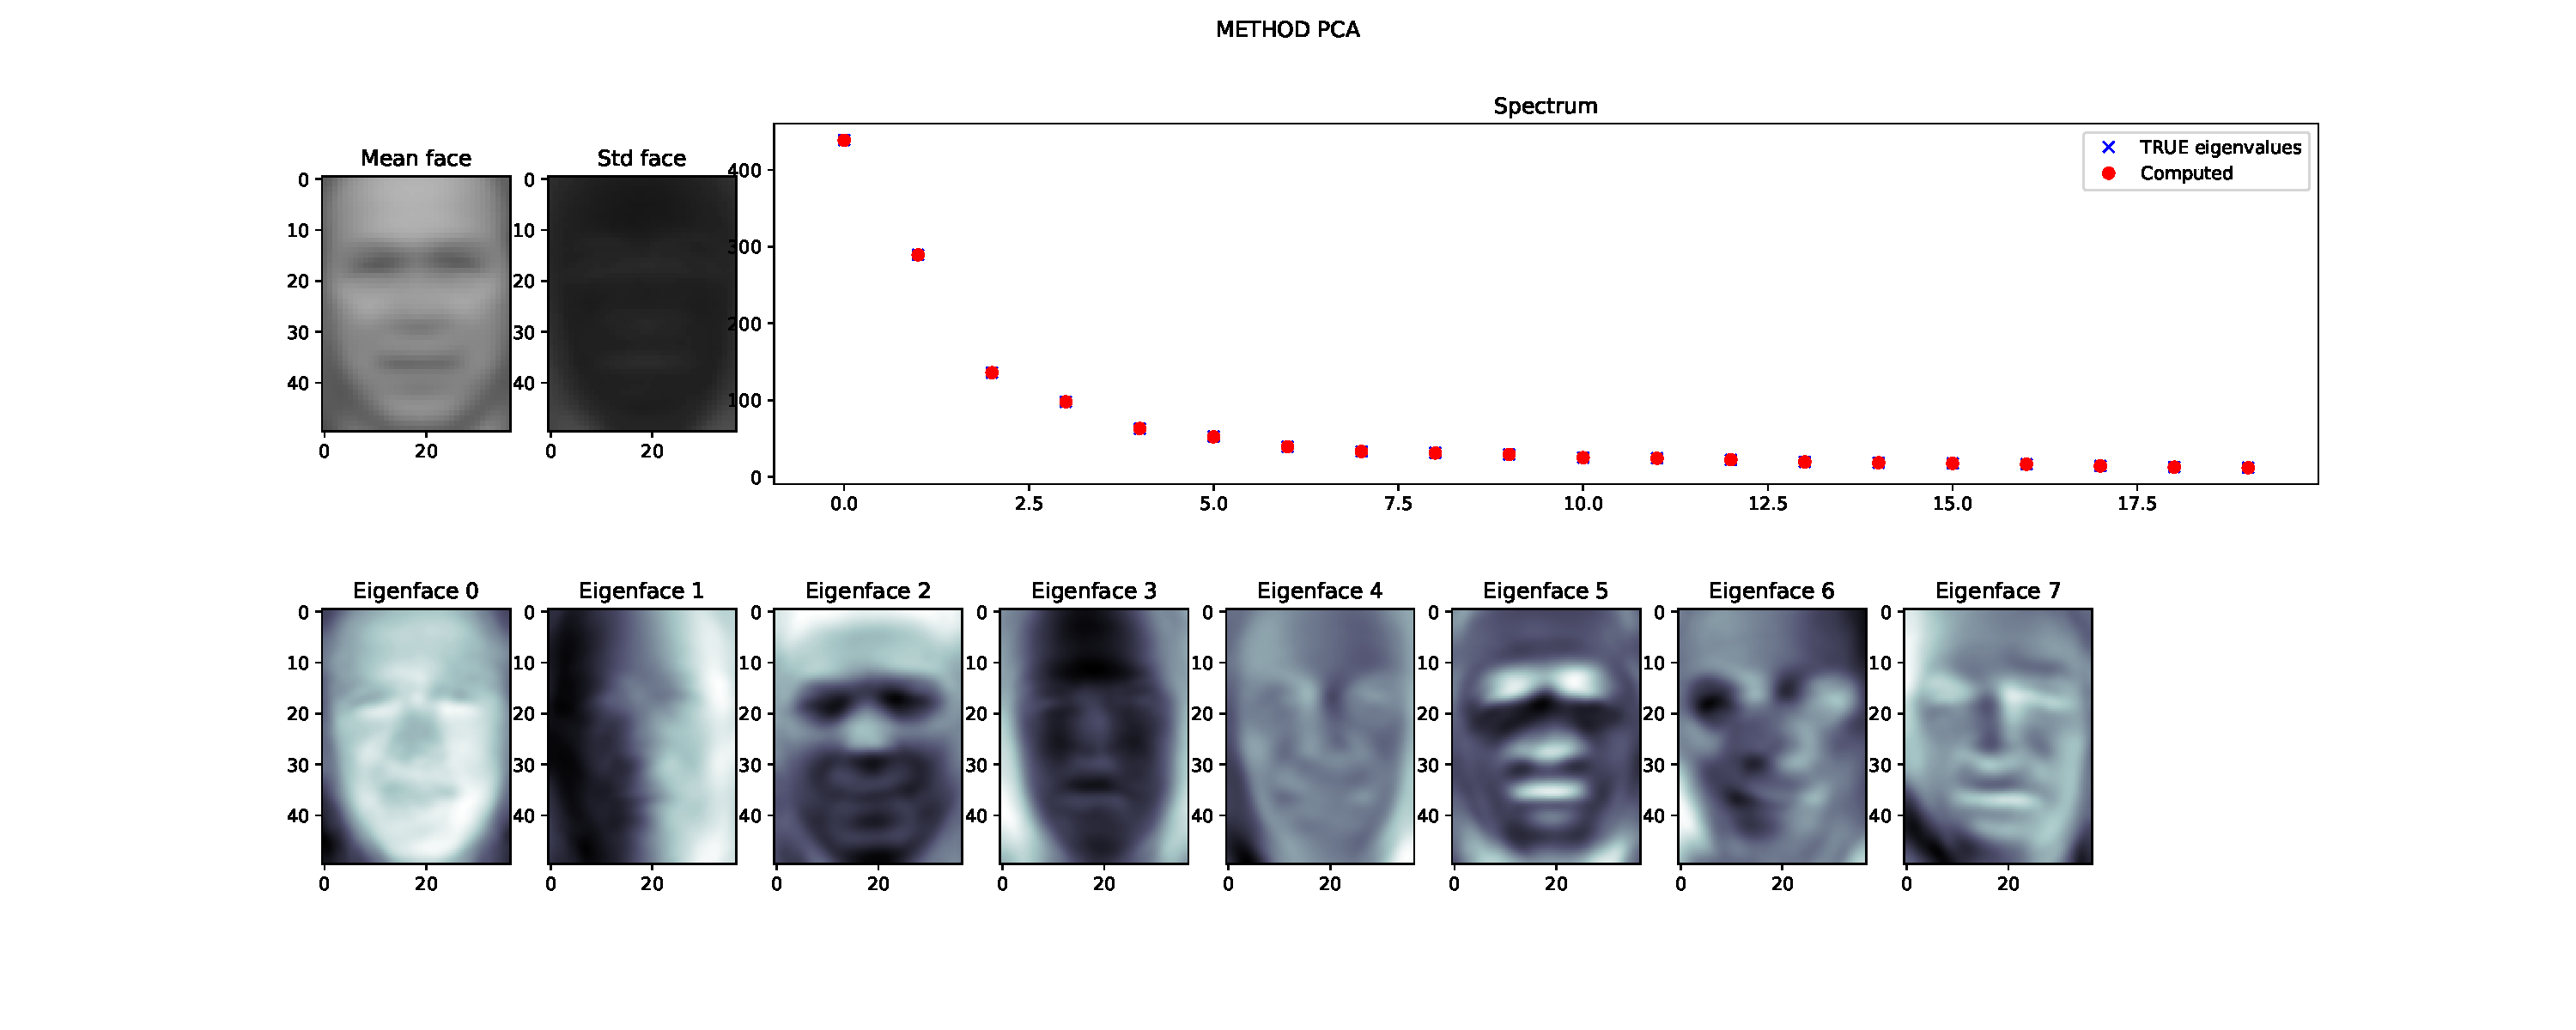
\includegraphics[width=\textwidth]{plots/faces_PCA_components.pdf}
    \caption{Values of the first 20 eigenvalues as well as the first 8 eigenfaces from our data set, calculated with our C++ code.}
    \label{fig:faces_comp}
  \end{minipage}
  \hfill
  \begin{minipage}[t]{0.7\textwidth}
    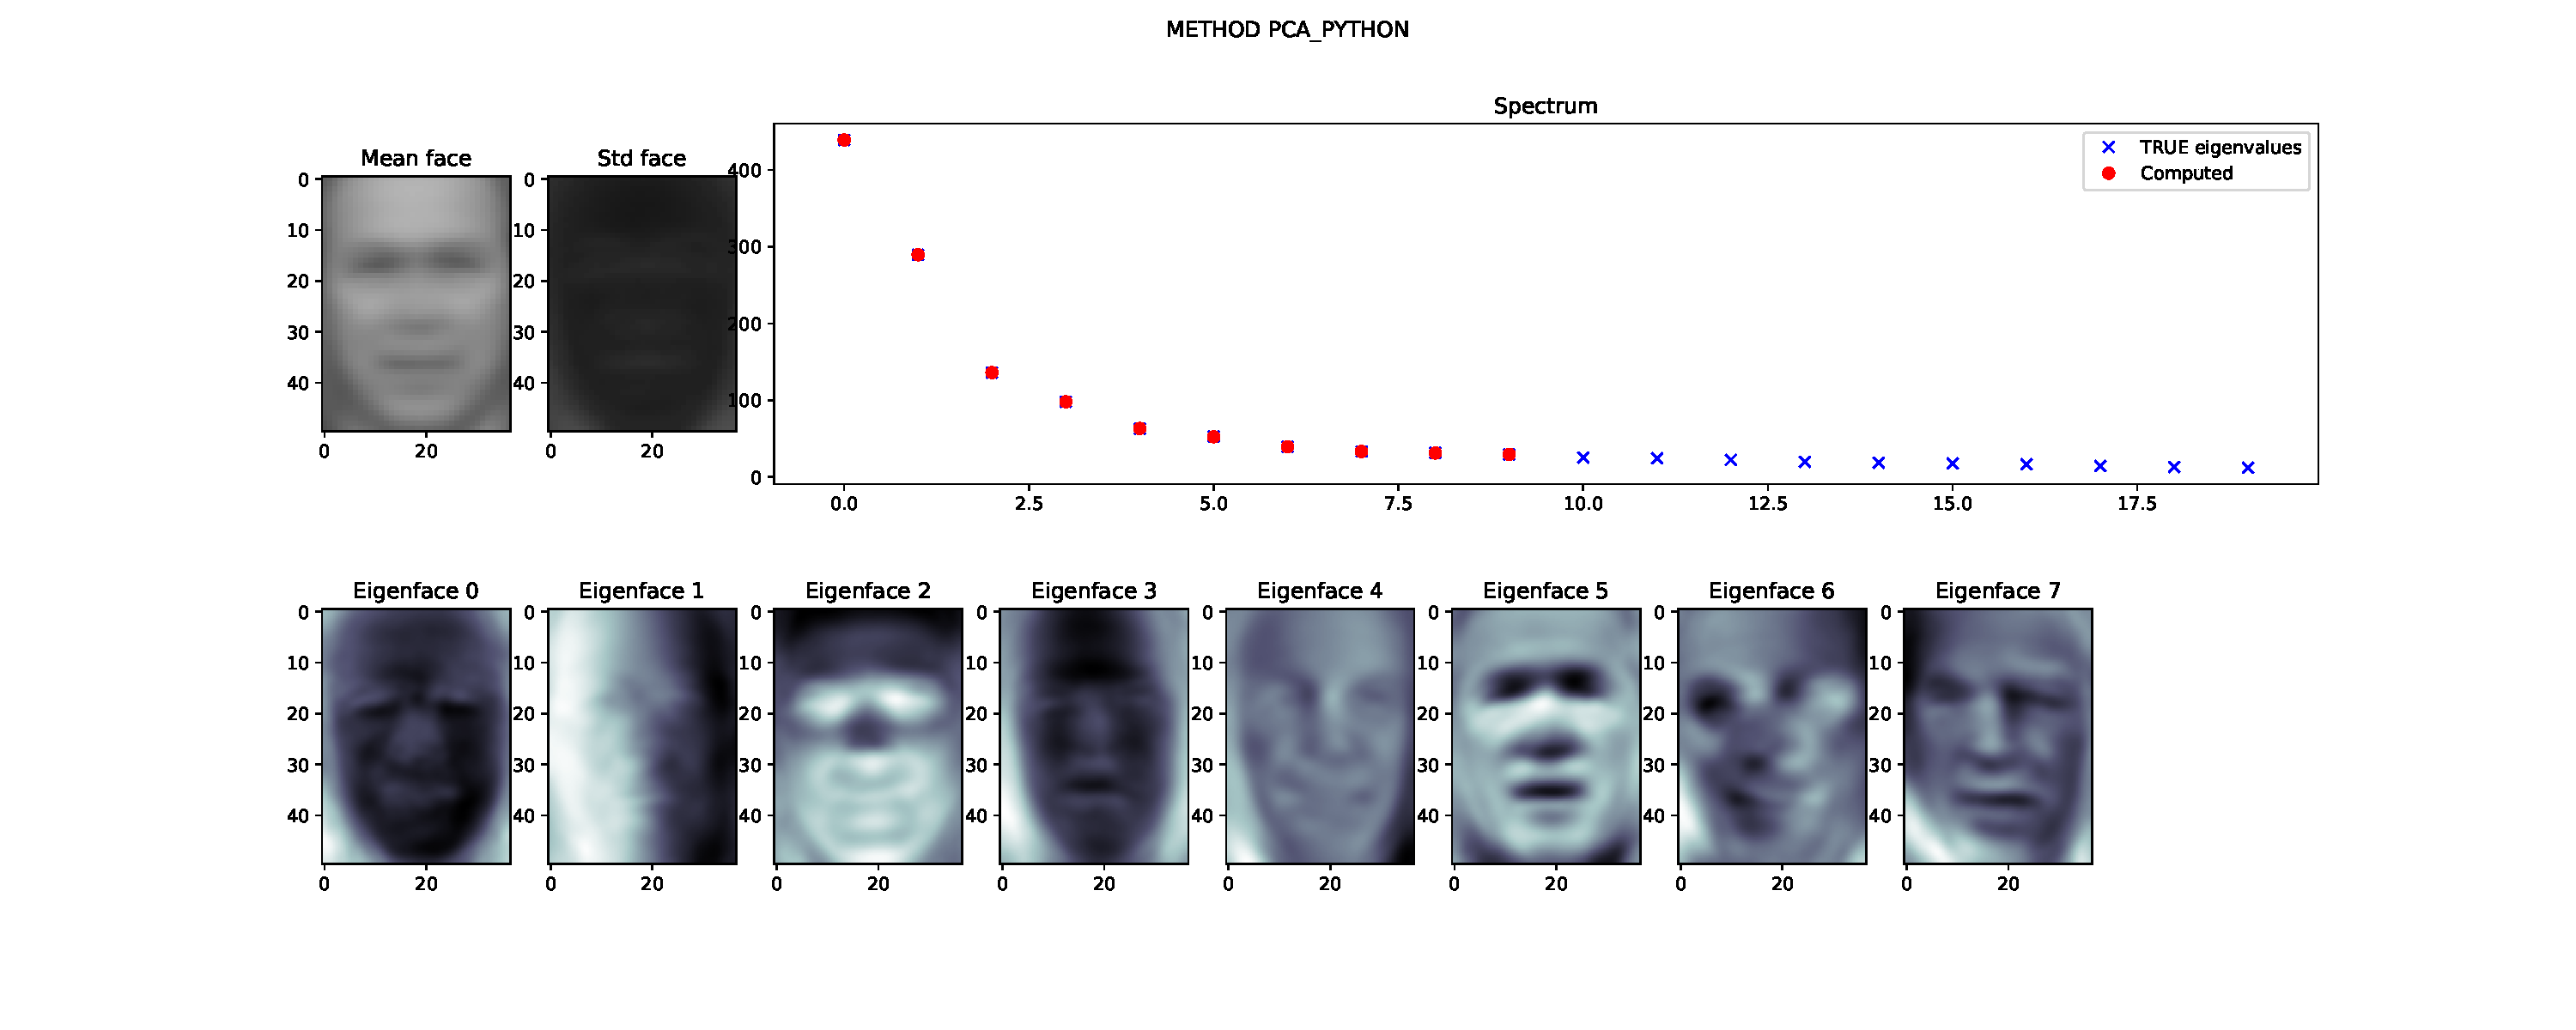
\includegraphics[width=1\textwidth]{plots/faces_PCA_PYTHON_components.pdf}
    \caption{Values of the first 20 eigenvalues as well as the first 8 eigenfaces from our data set, calculated with the reference Python code.}
    \label{fig:faces_comp_python}
  \end{minipage}
\end{figure}

\begin{figure}[h]
  \centering
  \begin{minipage}[t]{0.7\textwidth}
    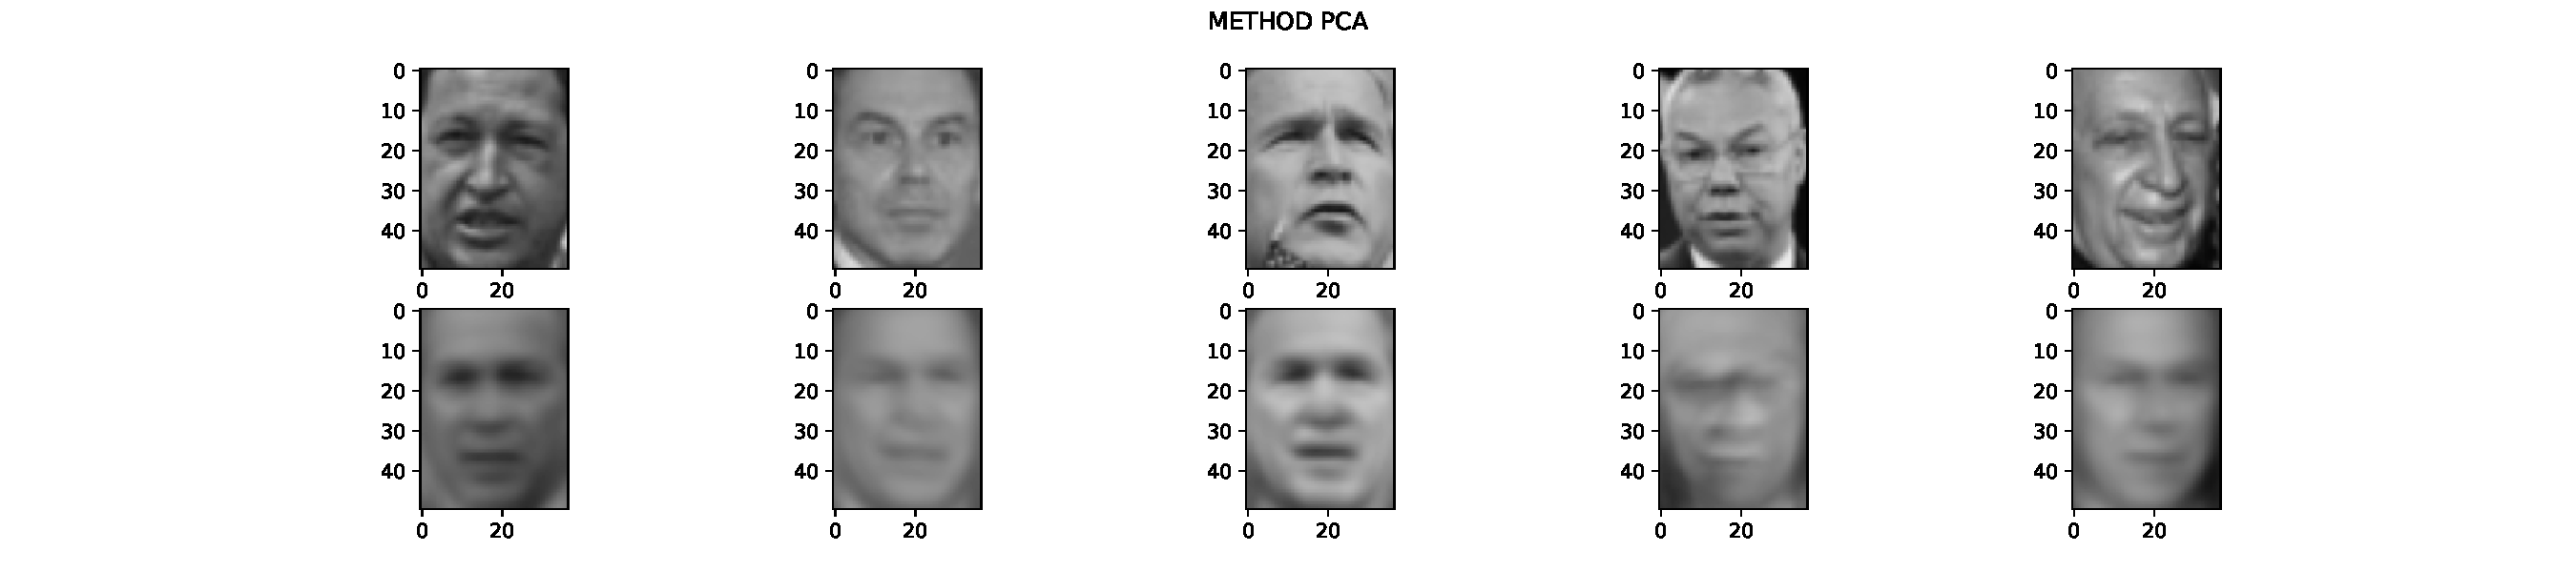
\includegraphics[width=\textwidth]{plots/faces_PCA_reconstruction.pdf}
    \caption{Values of 5 faces from our dataset as well as the reconstruction after PCA with 10 components, calculated with our C++ code.}
    \label{fig:faces_recon}
  \end{minipage}
  \hfill
  \begin{minipage}[t]{0.7\textwidth}
    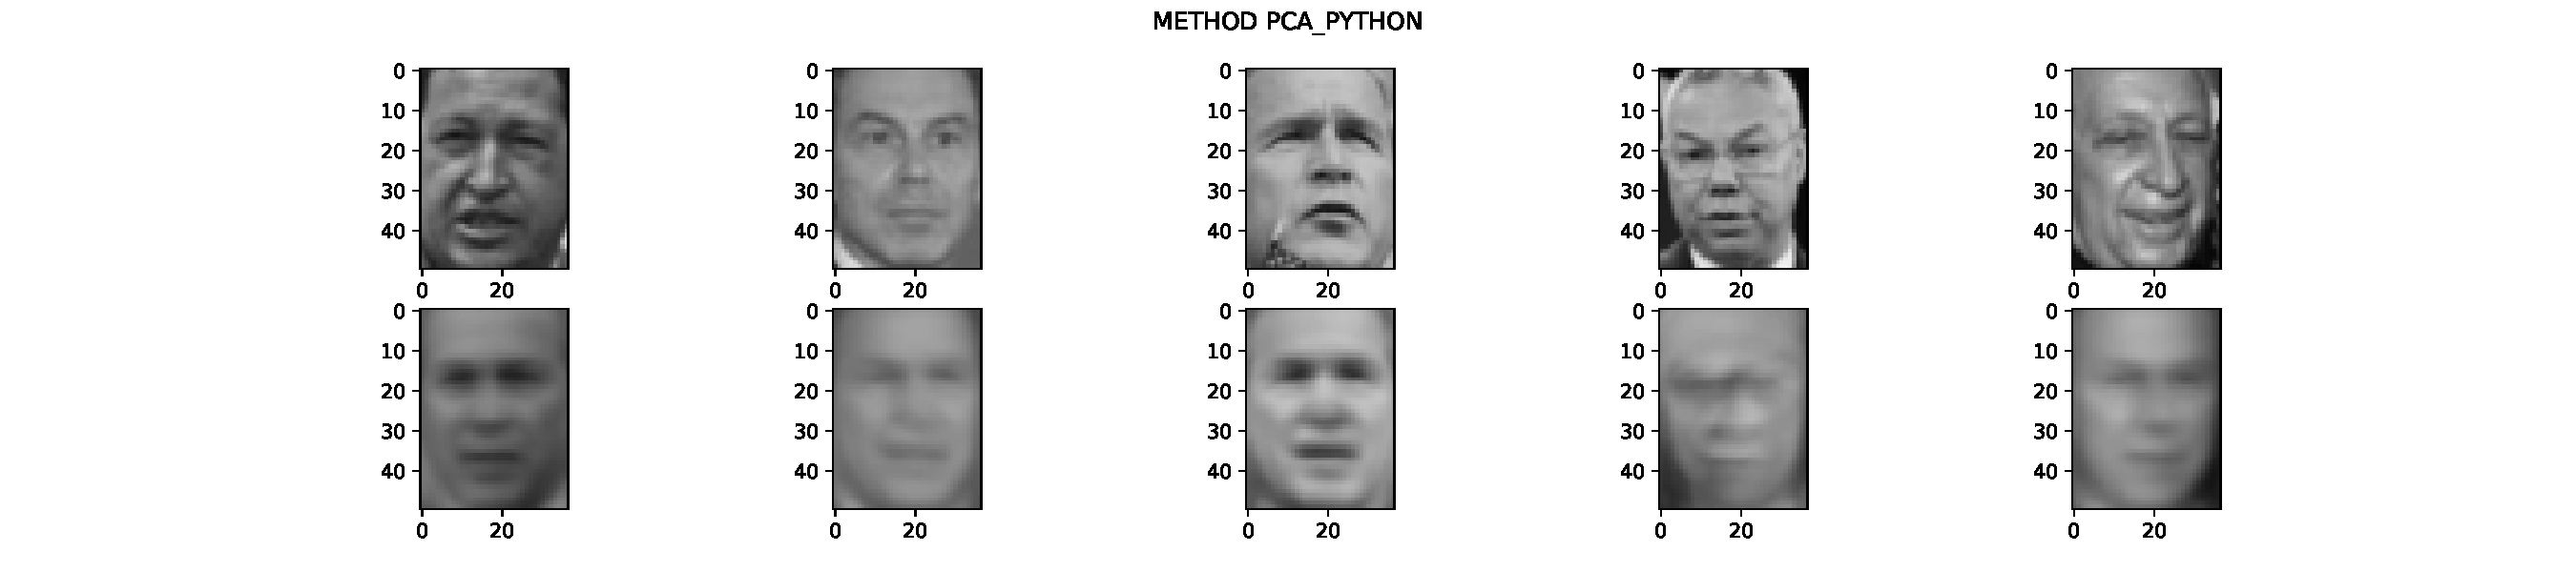
\includegraphics[width=1\textwidth]{plots/faces_PCA_PYTHON_reconstruction.pdf}
    \caption{Values of 5 faces from our dataset as well as the reconstruction after PCA with 10 components, calculated with the reference Python code.}
    \label{fig:faces_recon_python}
  \end{minipage}
\end{figure}

\section{Principal Component Analysis with Oja’s rule}
The eigenvalues retrieved from Hebb's rule are dependant on the number of iterations. With Hebb's rule our eigenvalues are diverging (going to $+\inf$), which is not well suited for our purpose. We also get the same eigenfaces for the principal components. With Oja's rule we don't have the problem of divergence anymore, but the issue of recovering the same principal components is still the same. Additionally, due to the stochastic nature of the algorithm (random weight initialization) we recover slightly different numerical results every time we run our code. The principal component we get from Oja's rule (and Hebb's rule) is similar to the one from the Python reference implemenation and the covariance implementation, though not completely the same. Interestingly enough the first principal component is the brightness of the face. We expect this to always be the first principal component, though the extent of it may vary due to several reasons, including numerical differences from the random weight initialization. 
For Sanger's rule we observe that it takes many iterations to attain good eigenvalues. While the first eigenvalue is similar to the reference implementation after a few hundred iterations, the other eigenfaces take significantly longer to attain similar values. We assume that the algorithm is unstable, as once can most probably find parameter combinations that will make the algorithm diverge or converge to a local minima rather than the global one (principal components). However, we didn't let our code run enough iterations in order to be able to find such scenarios. 

\begin{figure}[h]
  \centering
  \begin{minipage}[t]{0.7\textwidth}
    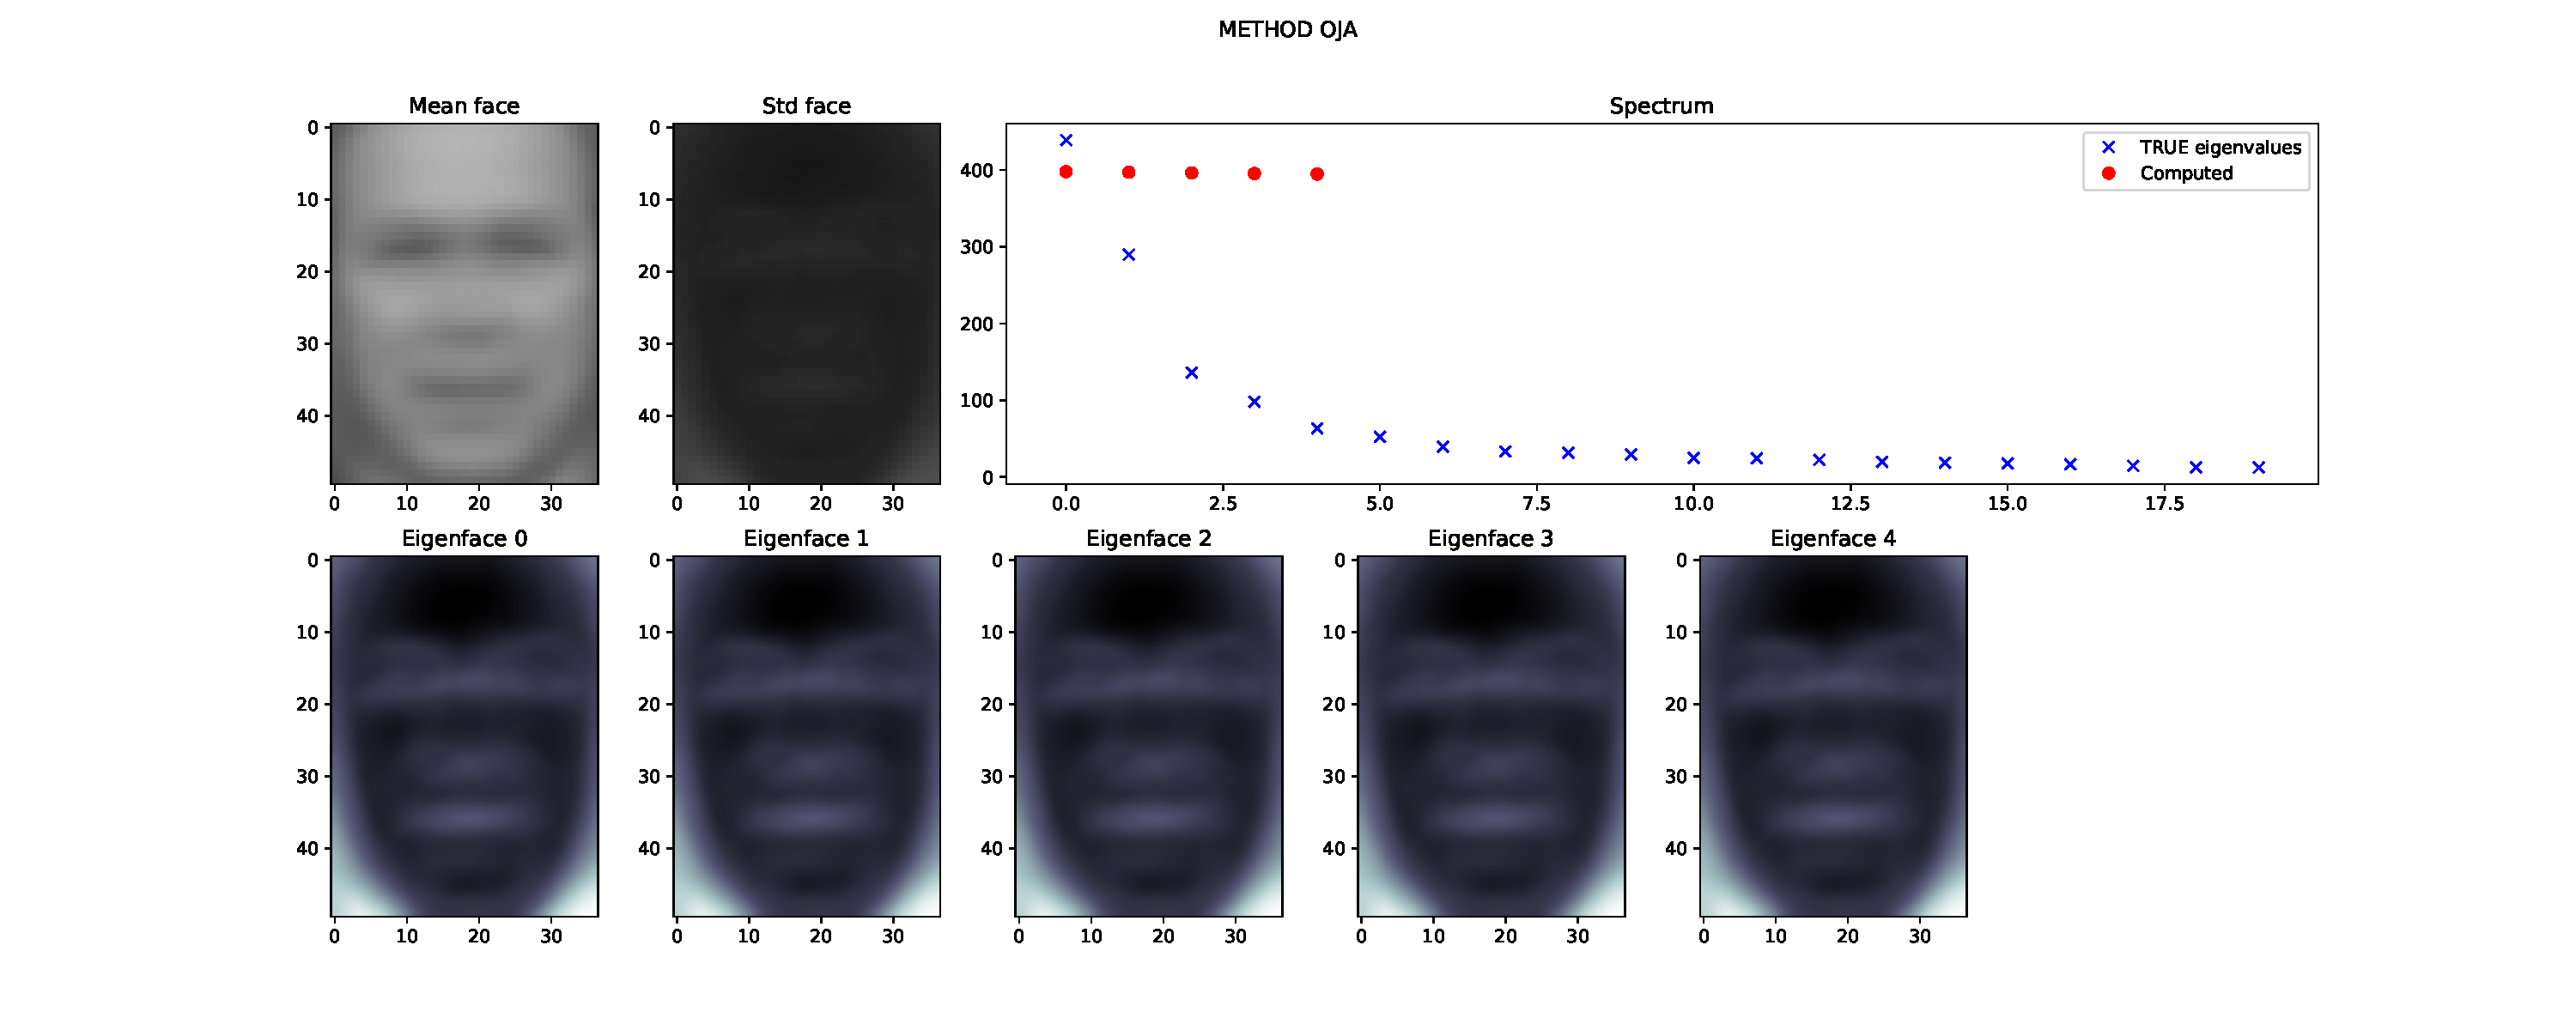
\includegraphics[width=\textwidth]{plots/faces_OJA_components.pdf}
    \caption{Values of the first 5 eigenvalues as well as the first 5 eigenfaces from our data set,, calculated with Oja's rule.}
    \label{fig:faces_recon}
  \end{minipage}
  \hfill
  \begin{minipage}[t]{0.7\textwidth}
    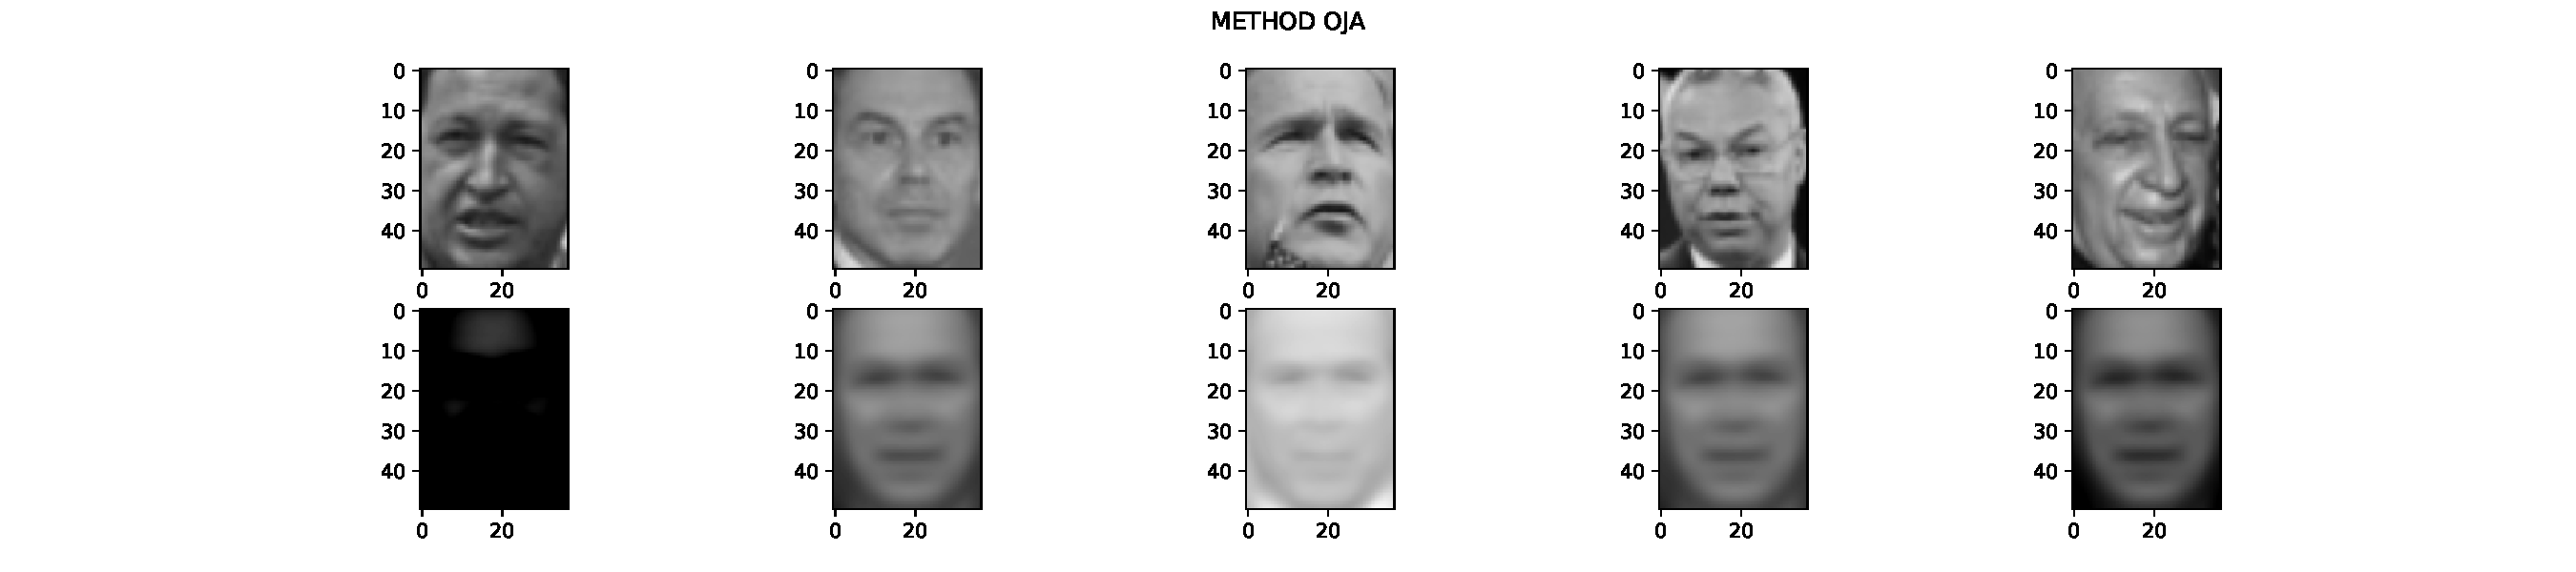
\includegraphics[width=1\textwidth]{plots/faces_OJA_reconstruction.pdf}
    \caption{Values of 5 faces from our dataset as well as the reconstruction after PCA with 5 components, calculated with Oja's rule.}
    \label{fig:faces_recon_python}
  \end{minipage}
\end{figure}

\bigskip
%----------------------------------------------------------------------------------------
%	REFERENCE LIST
%----------------------------------------------------------------------------------------

\printbibliography

%----------------------------------------------------------------------------------------

\end{document}

